\section{Generative Fitting} \label{sec:generative_fitting}

The generative fitting service is the most demanding procedure in the context of processing resources. The service represents the filtering and compression operations presented in Section \ref{sec:high_level_overview}. There are two scenarios based on the region's complexity. If the region is not complex, no further actions are taken except it formally was complex. Then, existing models have to be deleted, since they are not longer used. And if the region is complex, generative models are provided, which represent the exchange medium for information. More specifically, multiple \textit{Gaussian Mixture Models} (GMMs) are fitted on each label-subset of a region's data, which was stored in the indexing step in Section~\ref{sec:local_indexing}. According to a model selection process that evaluates the efficacy of each GMM, the best model is stored in the global pattern database, accessible to every member in the CIDS. The purpose of that elaborate process is that synthetic data can be sampled from these models. This way, every member has access to the global knowledge from all local infrastructures in order to enhance the local dataset that is used for fitting a classifier. Thus, this service is the key for providing \textit{privacy} and \textit{minimal overhead} while exchanging information.

\begin{algorithm}
    \caption{Retrieve Dataset from Region (Main Procedure)}
    \label{alg:generative_fitting}
    \algsetup{indent=2em}
 
    \begin{algorithmic}[1]
        \REQUIRE Regions $R_{\text{in}}$
        \ENSURE Regions $R_{\text{out}}$

        \STATE $m \leftarrow$ getID()
        \FORALL{$r$ in $R_{\text{in}}$}

            \STATE $k_\kappa \leftarrow \text{concatenate}(p_c, r)$
            \STATE $k_\delta \leftarrow \text{concatenate}(p_y, r, m)$

            \STATE $c_r \leftarrow PDB_G[k_\kappa]$
            \STATE $Y_r \leftarrow PDB_G[k_\delta]$ % get label set of region from global PDB

            \IF{$c_r = 0$}
                \FORALL{$y$ in $Y_r$}
                    \STATE $k_\omega \leftarrow \text{concatenate}(p_d, r, y, m)$ 
                    \STATE delete model in $PDB_G[k_\omega]$
                \ENDFOR
            \ELSE
                \STATE $L \leftarrow$ new List
                \FORALL{$y$ in $Y_r$}
                    \STATE $k_\alpha \leftarrow \text{concatenate}(p_x, r, y)$
                    \STATE $H \leftarrow PDB_{L_m}[k_\alpha]$
                    \STATE append $H$ to $L$
                \ENDFOR

                \STATE $D \leftarrow \text{preprocessing}(L)$

                \FORALL{$y$ in $Y_r$}
                    \STATE $\text{GMM} \leftarrow \text{modelSelection}(D, y)$
                    \STATE $k_\omega \leftarrow \text{concatenate}(p_d, r, y, m)$ 
                    \STATE $PDB_G[k_\omega] \leftarrow \text{GMM}$
                \ENDFOR
            \ENDIF
            


        \ENDFOR
    \end{algorithmic}
 \end{algorithm}

 First, regions that have been updated are received as events. As the data is further organized per label within a region, the labels for a region are retrieved. Then, if the region is not complex, no model fitting is executed. Instead, potentially existing models are deleted from storage. This is the case, if the complexity status of the has been changed from complex to simple.

 But if the region is complex, the generative model fitting procedure is triggered. Even if there are already models for the corresponding combination of region and label, an update of these models is initialized. For that, every hash table within a region, each containing data with a common label, is collected and added to a list. Subsequently, preprocessing operations prepare the collected region data for the model fitting. Details on the data preparation are described in Algorithm \ref{alg:data_preprocessing}.

 After that, the Model Selection process is started sequentially for each available label in the region. That way, the models are only fitted on data with the label in focus but evaluated with the complete region data. Specifics on the model selection are elaborated in Algorithm~\ref{alg:model_selection}. Finally, the best fitted model is stored in the global pattern database. So far, the main procedure has been outlined. Next, the details on the data preprocessing and the model selection are elaborated.

 \begin{algorithm}
    \caption{Preprocess Data}
    \label{alg:data_preprocessing}
    \algsetup{indent=2em}
 
    \begin{algorithmic}[1]
        \REQUIRE List of HashMaps $L$
        \ENSURE Dataset $D$
        
        \STATE $D \leftarrow \text{getValues(L)}$
        \FORALL{label in $D$}
            \IF{label $\neq 0$}
                \STATE \COMMENT{split into binary}
                \STATE $(X_a, y_a) \leftarrow (X, y)$ where $y=\text{label}$ 
                \STATE $(X_b, y_b) \leftarrow (X, y)$ where $y \neq \text{label}$
                \IF{$X.\text{shape}[0] < X.\text{shape}[1]$}
                    \STATE \COMMENT{upsample}
                \ENDIF
            \ENDIF
        \ENDFOR

    \end{algorithmic}
 \end{algorithm}

 Starting with the preprocessing.

 Splitting the dataset into a binary problem, such that the label that is currently in focus is the normal class and all other classes are attack classes. That way, the generative model can be evaluated using the machine learning efficacy method in the later course. 

 The upsampling process ensures that the fitting algorithm for the GMM is able to work. In practice, the number of samples has to be at least equal to the number of components. As some label subsets of a region may exhibit a low number of samples, in extreme cases only a single sample, an upsampling process is implemented. In particular, a set of nearest neighbours is generated per sample. First, the number of samples to generate is determined by the difference of the dimensionality of the data and the number of data points. Then, in order to generate from each data point equivalently, the number of nearest neighbours to sample is determined per data points. That is, the complete number of points to resample divided by the number of samples with an interger division (resulting in an integer). In case, the result of the interger division is zero, one is added to the result. Then for each data point $x$ in the set $X$, nearest neighbours are generated by sampling from a uniform distribution. This is done by considering each feature value of $x$ individually, such that the nearest neighbour is the concatenation of the sampled feature values as $x^* = [p(x_1), p(x_2), \dots, p(x_M)]$, where $p(x_m)=\frac{1}{b-a}$ within the interval $[x_m-\delta, x_m+\delta)$. The value $\delta$ controls the interval of the uniform distribution. The larger the value for $\delta$, the further the newly generated values deviate from the orginal feature values.


 \begin{figure}
    \centering
    \begin{subfigure}[b]{0.45\textwidth}
        \centering
        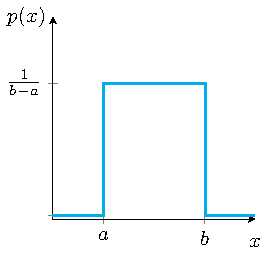
\includegraphics[width=\textwidth]{tikz/uniform_distribution.pdf}
        \caption{The probability density function of a uniform distribution is $p(x) = \frac{1}{b-a}$ within the interval $[a, b)$, and zero elsewhere.}
        \label{subfig:uniform_dist}
    \end{subfigure}
    \hfill
    \begin{subfigure}[b]{0.45\textwidth}
        \centering
        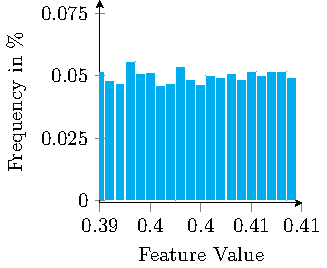
\includegraphics[width=\textwidth]{tikz/histogram_nearest_neighbour.pdf}
        \caption{Histogram of \numprint{10000} samples drawn from a uniform distribution over the interval $[x-\delta, x+\delta)$ where $x=0.4$ and $\delta=1 \cdot 10^{-2}$.}
        \label{subfig:hist_nn}
    \end{subfigure}
    \caption{Nearest neighbours are generated by sampling each feature value from a the uniform distribution.}
    \label{fig:uniform_dist_nn}
\end{figure}

 \begin{algorithm}
    \caption{Upsampling}
    \label{alg:upsampling}
    \algsetup{indent=2em}
 
    \begin{algorithmic}[1]
        \REQUIRE Collection of datapoints $X$
        \ENSURE Upsampled collection of datapoints $X_{up}$
        \STATE nResample $\leftarrow X.\text{shape}[1] - X.\text{shape}[0]$ \COMMENT{Difference of dim($X$) and num($X$) to fill}
        \STATE nResamplePerX $\leftarrow$ nResample $// X.\text{shape}[0] + 1$
        \STATE $X^* \leftarrow \emptyset$
        \FORALL{$x$ in $X$}
            \STATE $x^* \leftarrow$ new Array
            \FORALL{$x_m$ in $x$}
                \STATE sample a new $x_m^*$ from $p(x_m)$ and insert into $x^*$
            \ENDFOR
            \STATE add $x^*$ to $X^*$
        \ENDFOR
        \STATE $X_{up} \leftarrow X \cup X^*$
        \RETURN $X_{up}$

    \end{algorithmic}
 \end{algorithm}

 \begin{algorithm}
    \caption{Model Selection}
    \label{alg:model_selection}
    \algsetup{indent=2em}
 
    \begin{algorithmic}[1]
        \REQUIRE List of HashMaps $L$
        \ENSURE Dataset $D$
    \end{algorithmic}
 \end{algorithm}


% ALGO 3.1: Dataset preprocessing
% catalogs = {}
% for label in dataset:
%   if label is not benign:
%           // split into binary (filter the label that is to be learned into on chunk and the rest into another chunk)
%           // upsample

% ALGO 3.2: Model Fitting and Selection
% n_components <- collection of params[1 - X.shape//2, 2er schritte]
% cov_types <- collection of params[spherical, diag, full]
% for each component in n_components:
%   for each cov_type in cov_types:
%       X_pca <- pca.fit_transform(X)
%       gmm.fit(X_pca)
%       bic <- gmm.bic(X_pca)
%       // evaluation step
%           - synth. samples from gmm (how many?)
%           - inverse transform pca on these samples
%           - create training dataset
%           - create testing dataset
%           - train DecisionTreeClassifier with train dataset
%           - test DTClf with test dataset
%           - write balanced accuracy score into catalog
%           - write bic into catalog
% sort list_of_gmms by bic (lowest is best)
% sort list_of_gmms by acc (highest is best)
% return best gmm
